\section{Ergebnis}

\subsection{Prototyp}
\label{sec:prototyp}
Unser Prototyp umfasst wie hinlänglich beschrieben drei Komponenten, den Web-Service, eine Smartphone- sowie eine Smartwatch-Anwendung. 

Entsprechend unserer definierten Anwendungsfälle (s. Kapitel \ref{sec:useCases}) kann man mit unserer Anwendung
\begin{itemize}
\item{die eigene Position auf einen Raum genau bestimmen,}
\item{Notizen in einem Raum anbringen und anzeigen,}
\item{Notizen mit Ereignissen verknüpfen und bei diesem zur Anzeige bringen und}
\item{angebrachte Notizen wieder löschen.} 
\end{itemize}

Bei unseren Anwendungsfällen war ursprünglichen angedacht ebenfalls ein Gegenstandstracking zu implementieren, mit dem es möglich sein sollte Gegenstände auf einen Raum genau zu lokalisieren. Uns fehlte an dieser Stelle leider die Zeit, um das Feature fertig zu stellen. Wir sind aber äußerst optimistisch, dass das Gegenstandstracking gut funktioniert hätte.

Die folgenden Screenshots zeigen die wesentlichen Ansichten unserer Anwendungen.

\subsubsection{Smartwatch}
Die Smartwatch-Anwendung besteht aus einer Ansicht, die ggf. mehrfach instantiiert wird. Diese unterscheidet sich leicht durch die Displayform der jeweiligen Uhr. Die Abbildungen \ref{fig:ScreenshotWatchEckig} und \ref{fig:ScreenshotWatchRund} zeigen wie die Notizendarstellung unseres Prototyps ausschaut.

\begin{figure}[H]
\centering

\includegraphics[width=0.3\linewidth]{../Bilder/ScreenshotWatchEckig}
\caption{Screenshot unserer Uhr mit eckigem Display}
\label{fig:ScreenshotWatchEckig}
\end{figure}

\begin{figure}[H]
\centering

\includegraphics[width=0.3\linewidth]{../Bilder/ScreenshotWatchRund}
\caption{Screenshot unserer Uhr mit rundem Display}
\label{fig:ScreenshotWatchRund}
\end{figure}

\subsubsection{Smartphone}
Unsere Smartphone-Anwendung besteht aus zwei Ansichten. Die Hauptansicht erlaubt es Notizen zu erstellen und zur Smartwatch zu schicken (s. Abb. \ref{fig:ScreenshotPhoneMainActivity}), während eine weitere Ansicht zur Steuerung des Messvorgang (s. Abb. \ref{fig:ScreenshotPhoneRoomScanner}) dient.
 
\begin{figure}[H]
\centering
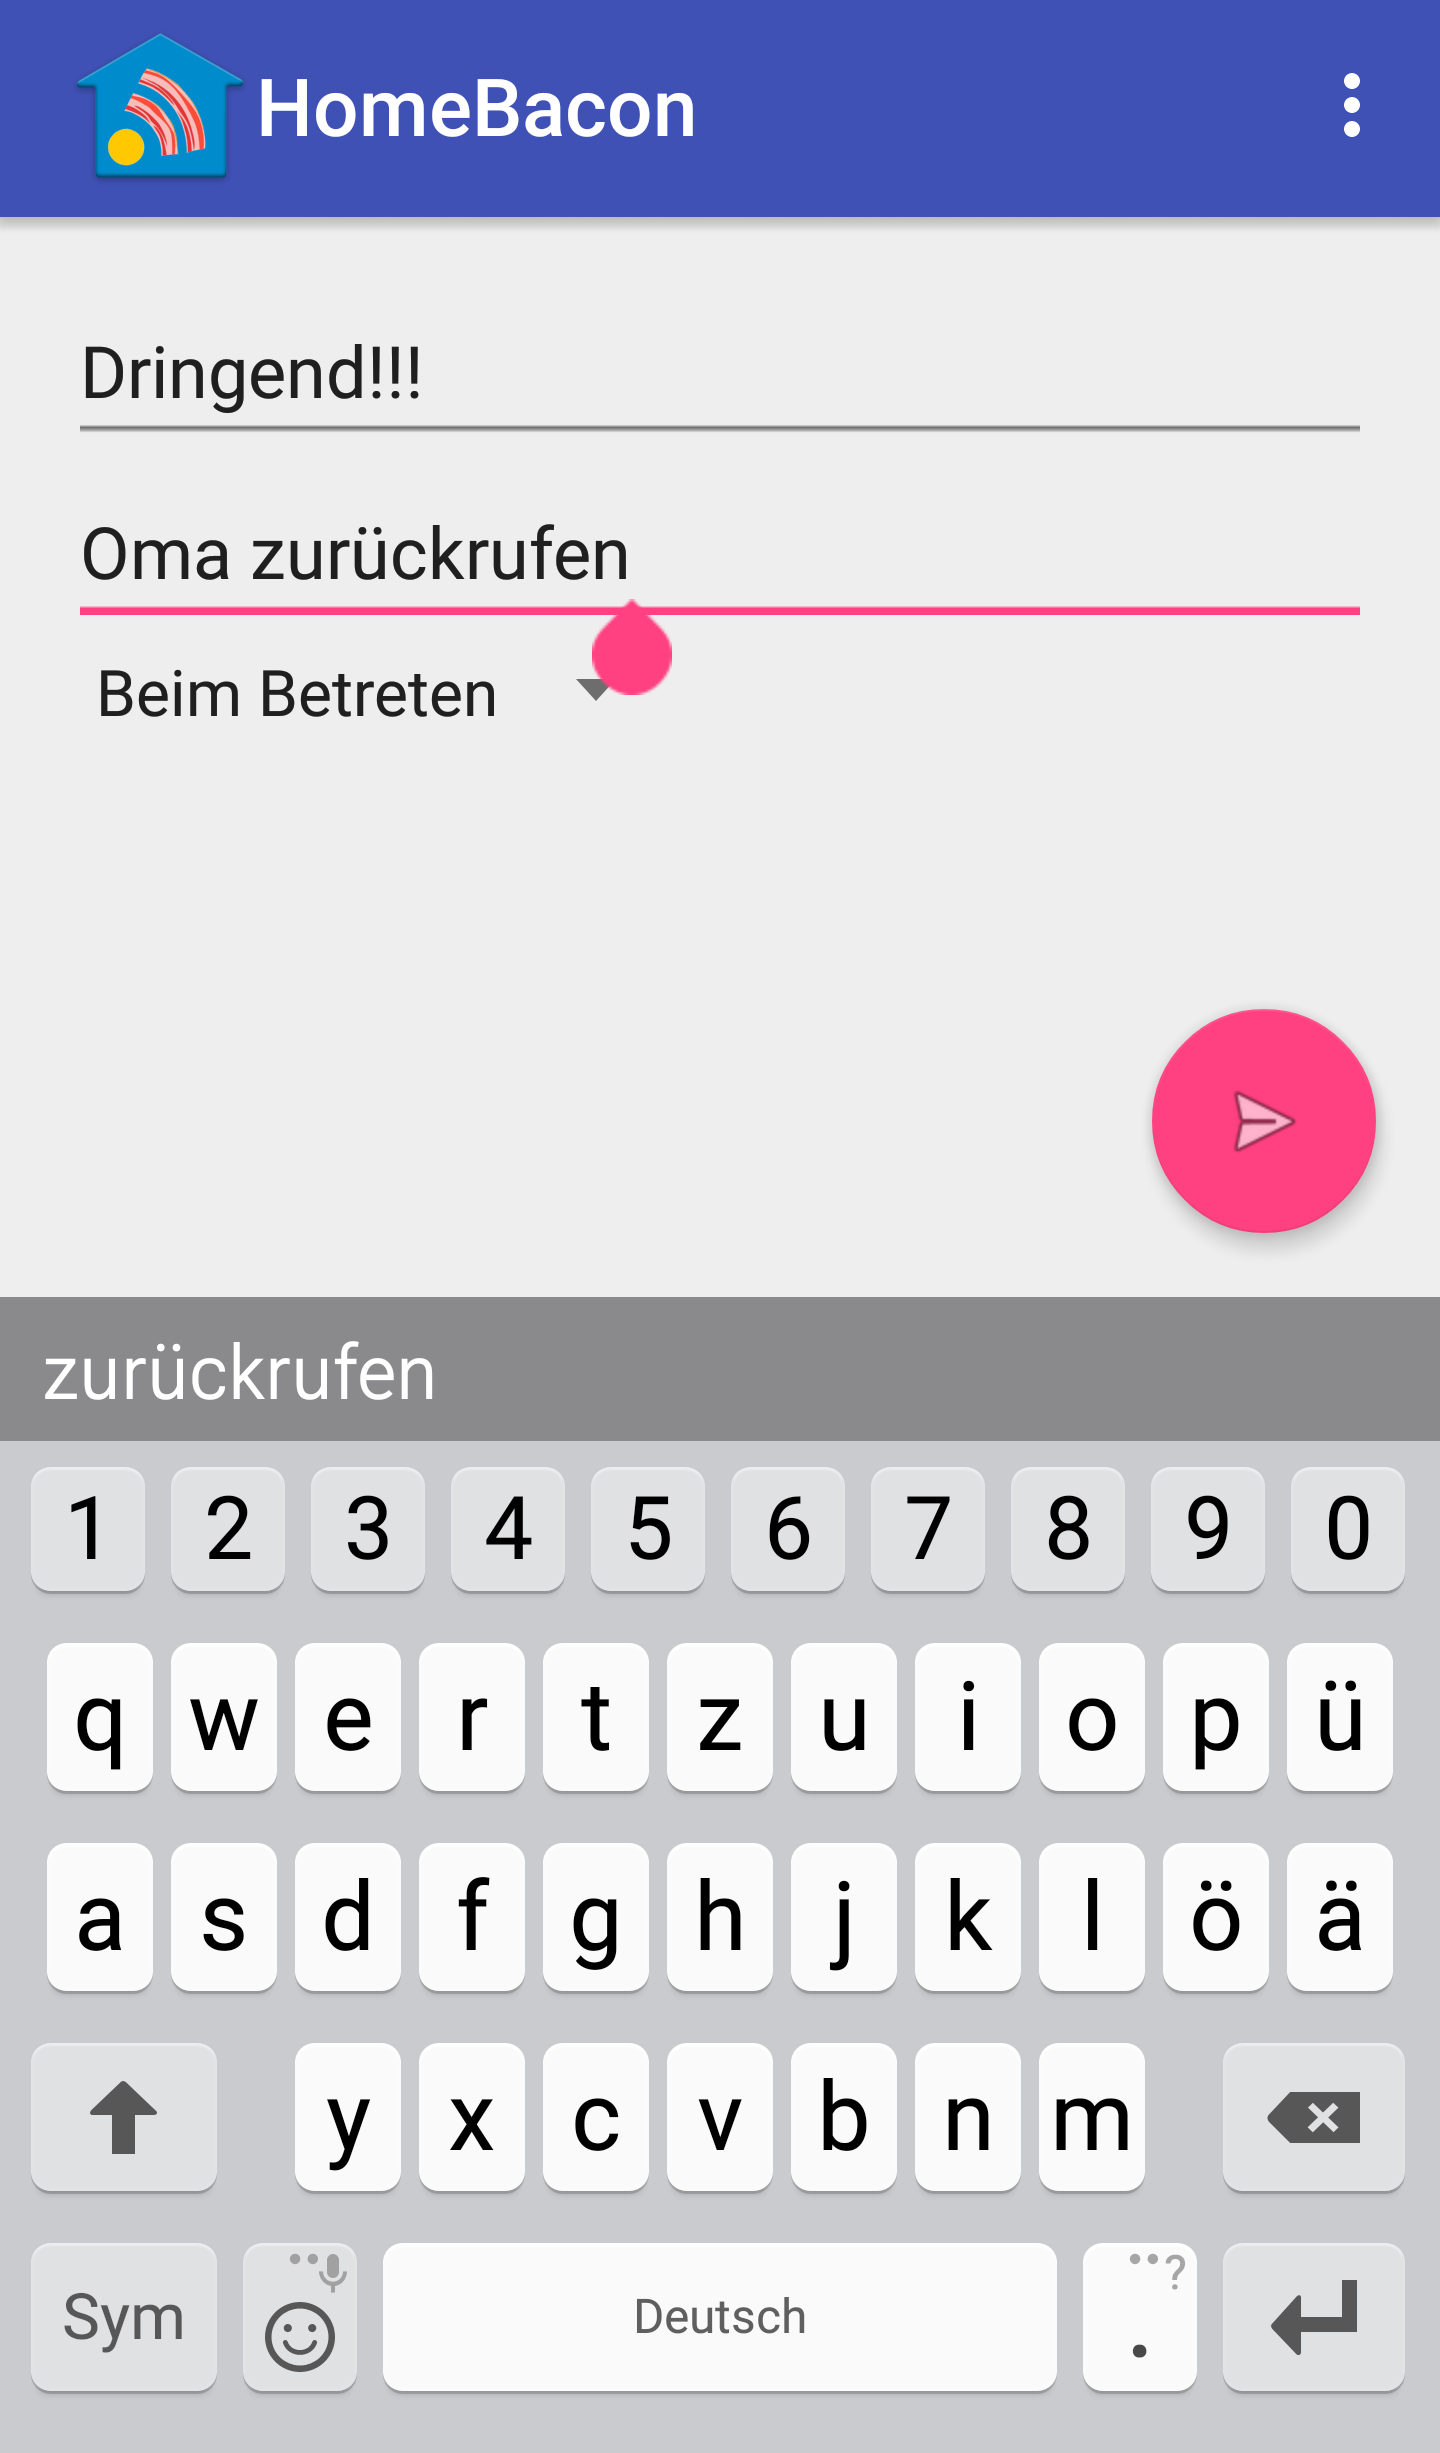
\includegraphics[width=0.4\linewidth]{../Bilder/ScreenshotPhoneMainActivity}
\caption{Screenshot der Ansicht zum erstellen von Notizen}
\label{fig:ScreenshotPhoneMainActivity}
\end{figure}

\begin{figure}[H]
\centering
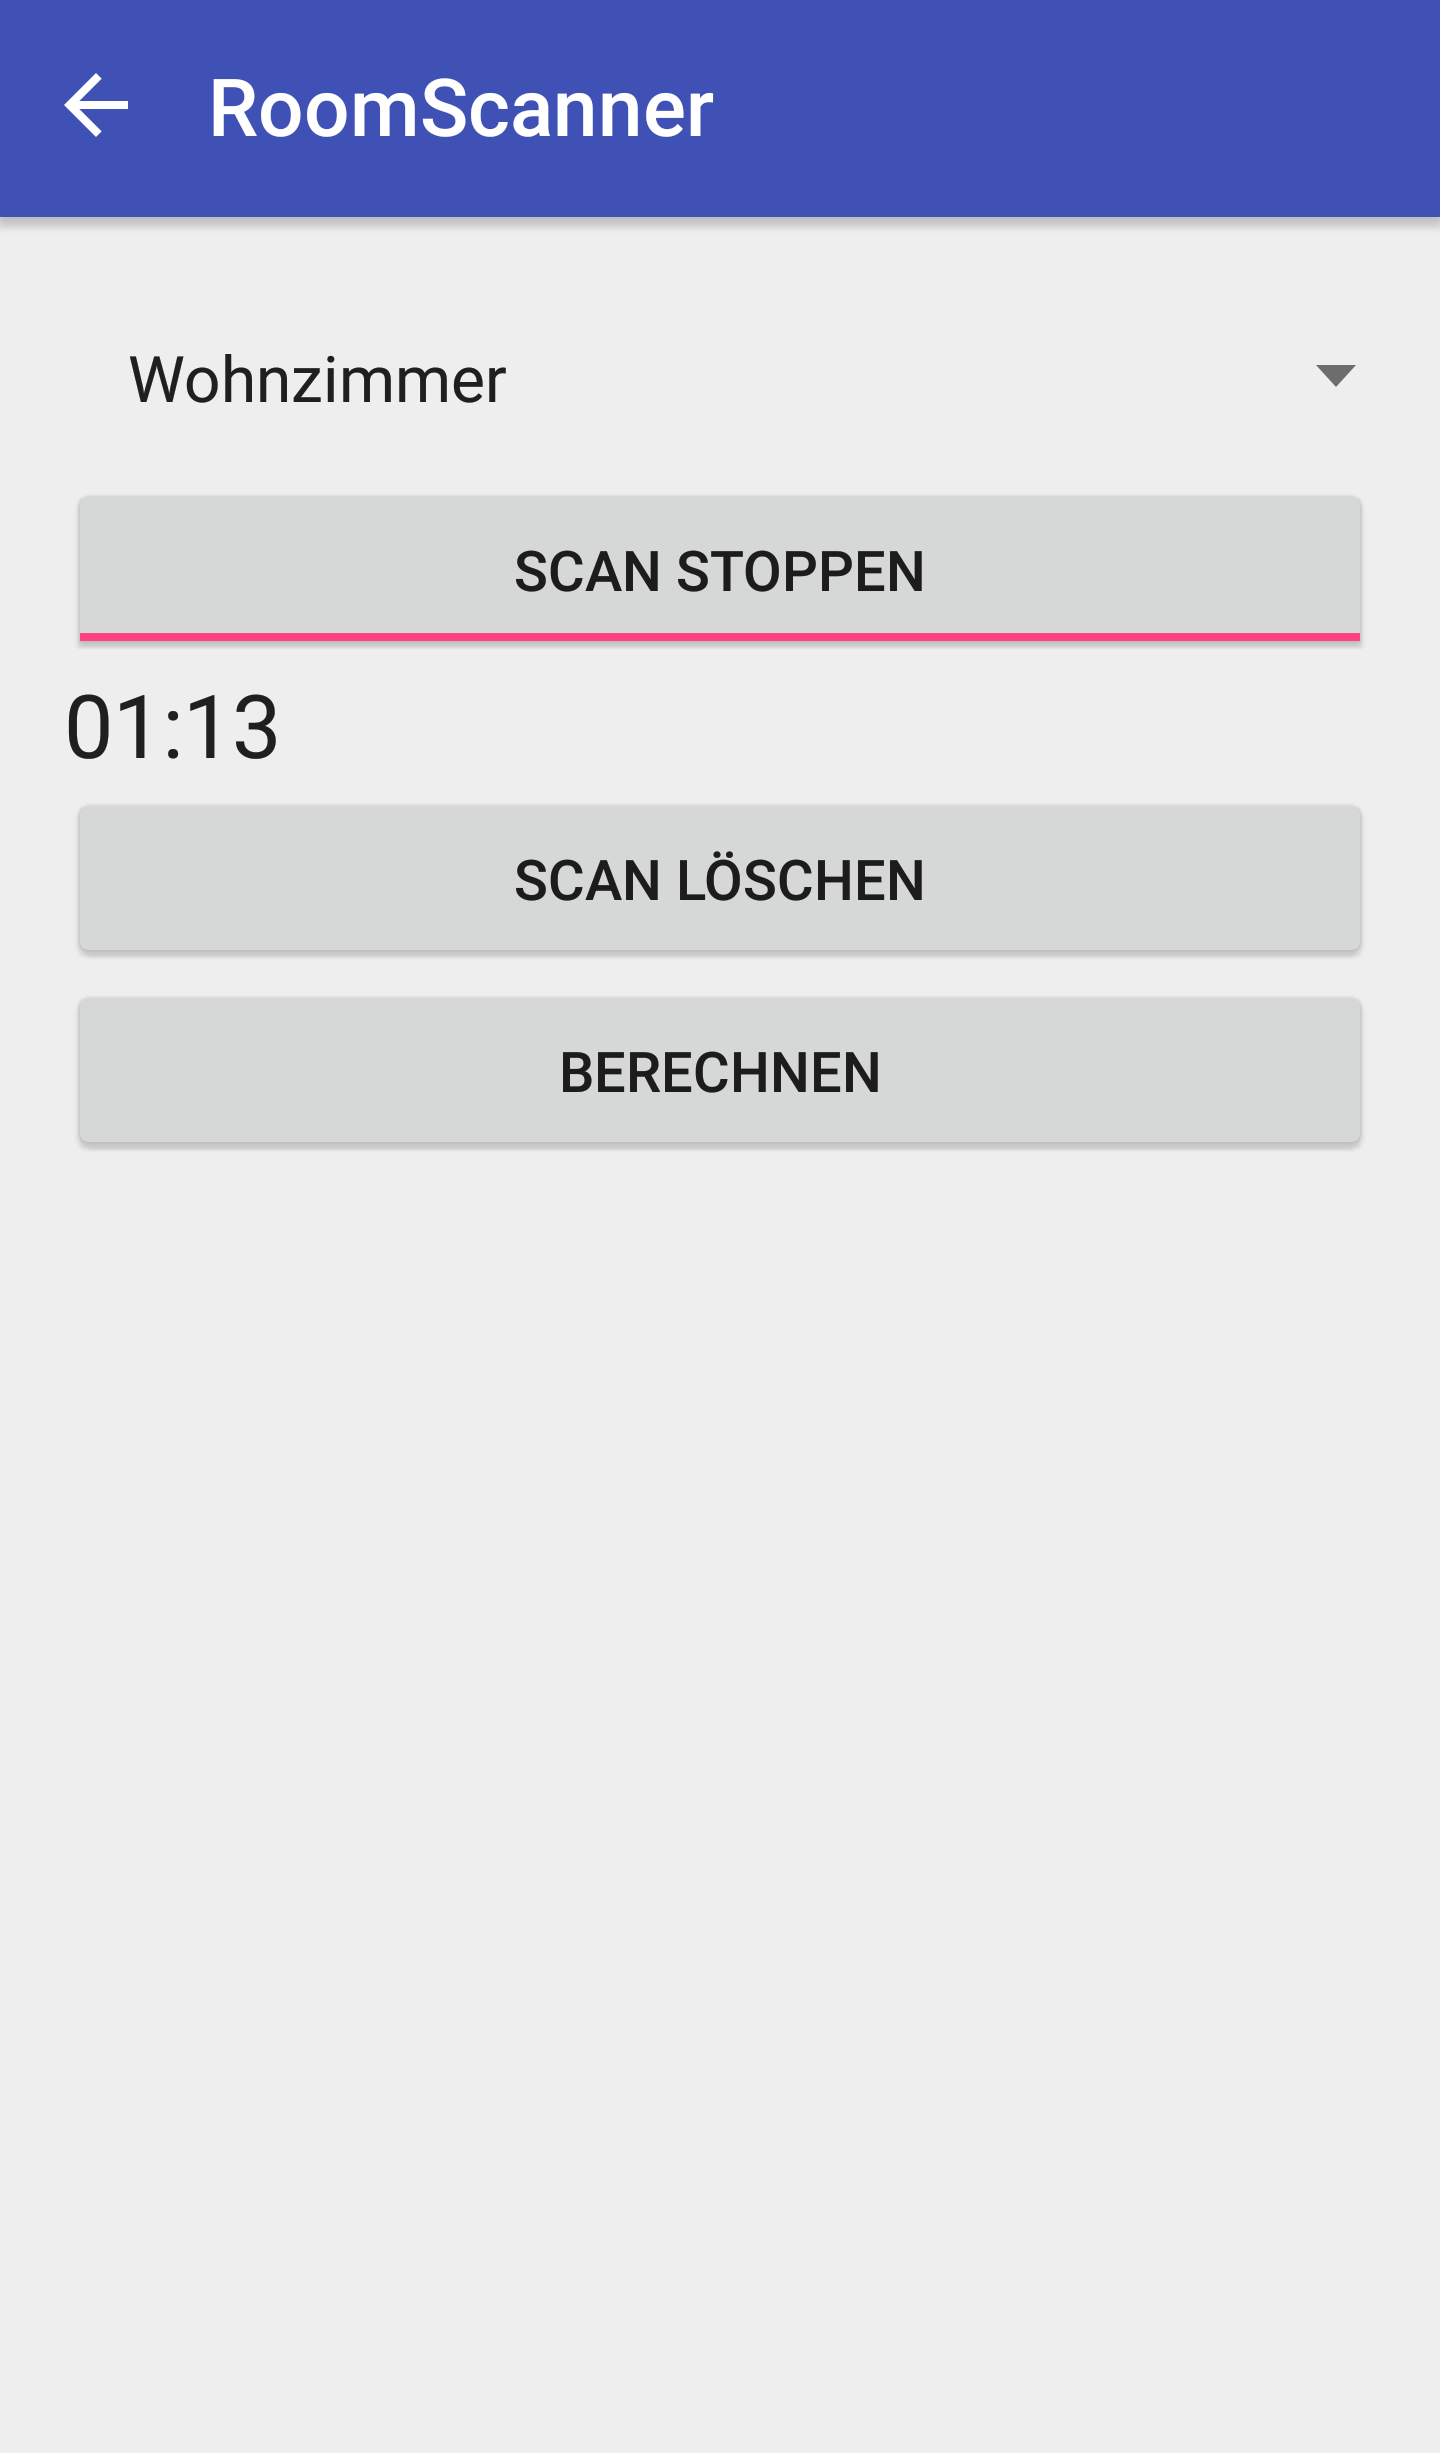
\includegraphics[width=0.4\linewidth]{../Bilder/ScreenshotPhoneRoomScanner}
\caption{Screenshot der Ansicht zum Vermessen von Räumen und erstellen}
\label{fig:ScreenshotPhoneRoomScanner}
\end{figure}



\subsection{Fazit}

Am Anfang dieses Projekts habe wir zuerst die Fragestellung genauer spezifiziert und erste Hardware Evaluationen vorgenommen. Diese Arbeitsschritte liefen weitgehend problemlos ab. Als Ergebnis daraus bestellten wir die fürs Projekt benötigte Hardware, bestehend aus 2 Smartwatches und 8 Bluetooth-Low-Energie-Beacons. Ein weiteres Resultat war ein Projektablauf Plan, der auch im laufe des Projekts eingehalten wurde und Anwendungsfalldiagramm, zur Strukturen und des Verhaltens unseres Prototypen. 

Im laufe der Entwicklung konnten wir große Erfahrungen im Umgang mit Android-Wear und das Entwickeln von Samrtwatch-Apps sammeln. Weiter war es uns möglich Fachübergreifendes Wissen aus Veranstaltungen wie "Artificial Intelligence - Künstliche Intelligenz" zu nutzen. Das half dabei die Raumerkennung über Bluetooth-Beacons zu realisieren.

Am Ende des Projekts hatten wir eine Android Wear Smartwatch-App, eine Android Smartphone-App und einen Web-Service. Die Smartwatch-App dient zu Darstellung von Notizen und zum messen der Bluetooth-Beacons. Die Samrtwatch-App startet und stoppt eine Messung, sowie ermöglicht sie das erstellen von Notizen und sendet und empfängt Daten vom Web-Service. Der Web-Service erhält Messungen und berechnet daraus das Model zur Raumbestimmung.

Mithilfe all dieser Komponenten ist es dann möglich eine Automatisierte Raumerkennung zu machen und virtuelle Notizen in Räume zu legen bzw. Notizen beim verlassen oder betreten eines Raumes anzuzeigen.
